\documentclass[a4]{article}
\usepackage{multicol}
\usepackage{graphicx}
\linespread{1.35}
\usepackage{amsmath}
\usepackage{color}
\usepackage{xcolor}
\usepackage{tikz}
\usetikzlibrary{arrows,automata}


\begin{document}


\begin{flushright}
 \textcolor{blue}{\hspace*{0.5cm} \texttt{Finite State Machine} \hspace*{0.10cm}\textbf{$|$} \textbf{157}\hspace*{0.5cm}}
\end{flushright}

\vspace*{1cm}
%paragraph 1 (پاراگراف اول)


The pair if states which are connected by undirected arcs(not crossed in the interrupted portion) are compatible pairs.

%paragraph 2 (پاراگراف اول)


The compatible pairs of the given machine are (AB), (AC), (AF), (BC), (BD), (BF), (CE), (cF), and (DE).

%paragraph 3 (پاراگراف اول)


Therefore, in the compatibility graph there are nine vertices.

%paragraph 4 (پاراگراف اول)


In the given machine,
\vspace*{0.10cm}

(BD) is the implied pair for (AB). So, a directed arc is drawn from (AB) to (BD).



%paragraph 5 (پاراگراف اول)

(CE) is the implied pair for (AF). So, a directed arc is drawn from (AF) to (CE).

%paragraph 6 (پاراگراف اول)


(DE) is the implied pair for (BC). So, a directed arc is drawn from (BC) to (DE).

%paragraph 7 (پاراگراف اول)


(BD) is the implied pair for (BD). As ($S_{i}$ , $S_{j}$) $\neq$ ($S_{p}$ , $S_{q}$), no arc is drawn from (BD) to (BD).

%paragraph 8 (پاراگراف اول)


(AC) and (BF) are implied pair for (DE). So, two directed arcs is drawn from (DE) to (AC) and (BF).

%paragraph 9 (پاراگراف اول)


The compatibility graph for the given machine is given in Fig.4.17.



\begin{center}
  \section{picture}
\includegraphics[width=6cm,height=6cm]{157.png}
\end{center}
\textcolor{red}{\centerline{\textbf{Fig.4.16} \hspace*{0.5cm} \texttt{Merger Graph}}}

\vspace*{1cm}

\fcolorbox{blue}{yellow}{\textbf{4.7.4 \hspace*{0.5cm} \texttt{Minimal Machine Construction}}}
\vspace*{0.2cm}


To construction the minimal machine, a compatible graph construction is an essential part. After this, we have to find closed compatible, closed covering, and from there mini-mal closed covering.

%paragraph 10 (پاراگراف اول)


A subgraph of a compatibility graph is called closed if, for every vertex in the subgraph, all outgoing arcs and the terminal vertices of the arcs also belong to the subgraph. The pair of states that belong to the subgraph as terminal vertices are called closed compatible.


%paragraph 11 (پاراگراف اول)


if a subgraph is closed, and if every state of the machine is covered by at least one vertex of the sub-graph of a compatibility graph, then the subgraph forms a closed covering of the machine.

%paragraph 12 (پاراگراف اول)


To find a minimal machine, we need to find the subgraphs which closed cover the machine. Then, we need to find the subgraph which contains less number of vertices and which can generate a simpler machine. The states of the minimal machine are the vertices of the subgraph. Fromthese states, the tran-sition functions are constructed. By this process, a minimal machine of the given machine is constructed.

%paragraph 13 (پاراگراف اول)


The minimal machine is constructed by the following process for the machine given as an example in the compatibility graph section.
\vspace*{0.5cm}

\begin{center}
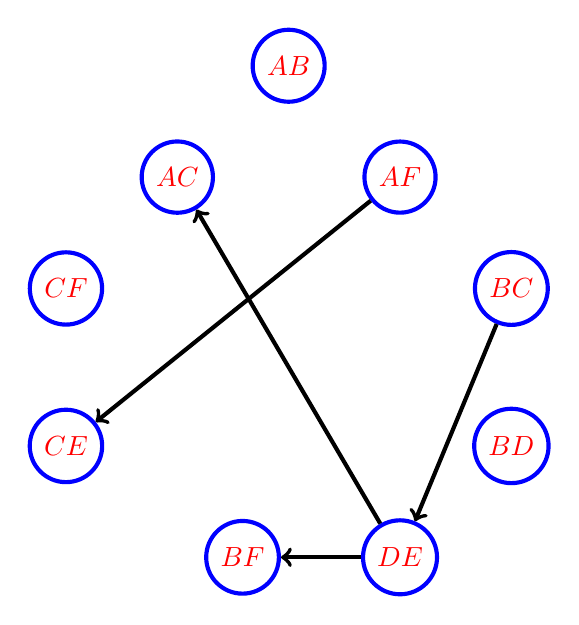
\begin{tikzpicture}[->,node distance = 2cm,line width=1.5pt]
\node[state,text=red,draw=blue] (A) {$AB$};
\node[state,text=red,draw=blue] (B) [below left of = A] {$AC$};
\node[state,text=red,draw=blue] (C) [below left of = B] {$CF$};
\node[state,text=red,draw=blue] (D) [below right of = A] {$AF$};
\node[state,text=red,draw=blue] (E) [below right of = D] {$BC$};
\node[state,text=red,draw=blue] (G) [below of = E] {$BD$};
\node[state,text=red,draw=blue] (I) [below left of = G] {$DE$};
\node[state,text=red,draw=blue] (F) [below of = C] {$CE$};
\node[state,text=red,draw=blue] (H) [left of = I] {$BF$};
\path (D) edge (F);
\path (E) edge (I);
\path (I) edge (H);
\path (I) edge (B);

\end{tikzpicture}
\end{center}

\textcolor{red}{\centerline{\textbf{Fig.4.17} \hspace*{0.5cm} \texttt{Compatible Graph}}}
\vspace*{1cm}


\fcolorbox{blue}{yellow}{\textbf{4.7.5 \hspace*{0.5cm} \texttt{Minimal Machine}}}
\vspace*{0.2cm}


The subgraphs (AC), (DE), (BF) or (AB), (BD), (AF), (CE) or (AF), (CE), (BC), (DE) are closed subgraphs  of the compatibility graph and forms a closed cover of the machine (here every state of the machine is covered by at least one vertex of the subgraph). Among them, the subgraph (AC)(DE)(BF) contains less number of vertices.

%paragraph 14 (پاراگراف اول)


In the minimal machine, the states are (AC), (BF), and (DE).Let us rename them as $S_1$,$S_2$,$S_3$, respec-tively. The minimal machine becomes

\newpage
  \begin{flushleft}
 \textcolor{blue}{\textbf{158}\hspace*{0.1cm} \textbf{$|$} \hspace*{0.1cm} \texttt{Introduction to Automata Theory, Formal Languages and Computation}}
  \end{flushleft}

\vspace*{2cm}

\begin{center}
\begin{tabular}{ccccc}
 \hline

 \hline

 \hline

 \hline

\multicolumn{5}{c}{$Next State, z$}\\
 \cline{2-5}
       $Present State$   &    $I_1$      &    $I_2$        &        $I_3$   &     $I_4$      \\
 \hline
       $S_1(AC)$         &    $S_3, 1$   &     $S_1, 1$    &     $S_3, 0$   &   $S_2, 1$     \\
       $S_2(BF)$         &    $S_1, 1$   &     $-, -$      &     $S_3, 0$   &   $S_3, 1$      \\
       $S_3(DE)$         &    $S_1, 0$   &     $S_2, 1$    &     $S_2, 0$   &   $S_3, 0$     \\
 \hline

 \hline

 \hline

 \hline
\end{tabular}
\end{center}

\fcolorbox{red}{pink}{\textbf{Example 4.11}} \hspace*{0.1cm} \texttt{Draw a compatible graph for the following machine. Hence, find the minimal machine.}

\vspace*{0.2cm}
\large{\textbf{Solution:}}

\vspace*{0.1cm}

\begin{center}
\begin{tabular}{ccccc}
 \hline

 \hline

 \hline

 \hline

\multicolumn{5}{c}{$Next State, z$}\\
 \cline{2-5}
       $Present State$   &    $I_1$      &    $I_2$        &        $I_3$   &     $I_4$      \\
 \hline
       $A$         &    $-,-$    &     $D, 0$    &     $D, 0$   &   $C, -$     \\
       $B$         &    $A, 1$   &     $-, -$    &     $-, -$   &   $D, -$     \\
       $C$         &    $B, 1$   &     $C, 0$    &     $E, 0$   &   $-, -$     \\
       $D$         &    $E, 1$   &     $C, 0$    &     $-, -$   &   $D, 0$     \\
       $E$         &    $-, -$   &     $-, -$    &     $-, -$   &   $A, 1$     \\
 \hline

 \hline

 \hline

 \hline
\end{tabular}
\end{center}

\hspace*{0.2cm} To find the compatible pairs of a machine, we need to construct the merger graph first. According
to the rules for the construction of the merger graph, the following graph as shown in Fig. 4.18 is constructed.


\begin{center}
  \section{picture}
\includegraphics[width=4cm,height=4cm]{158.png}
\end{center}
\textcolor{red}{\centerline{\textbf{Fig.4.18} \hspace*{0.5cm} \texttt{Merger Graph}}}

\hspace*{0.2cm} The pair of states which are connected by undirected
arcs (not crossed in the interrupted portion) are compatible
pairs.\\

\hspace*{0.2cm} The compatible pairs of the given machine are (AB),
(AD), (BC), (BE), (CD), and (CE). Therefore, in the
compatibility graph of the previous machine, there are
nine vertices.\\

\hspace*{0.2cm} (CD) is the implied pair for (AB). A directed arc is
drawn from (AB) to (CD).\\

\hspace*{0.2cm} (CD) is the implied pair for (AD). A directed arc is
drawn from (AD) to (CD).\\

\hspace*{0.2cm} (AB) is the implied pair for (BC). A directed arc is
drawn from (BC) to (AB).\\

\hspace*{0.2cm} (AD) is the implied pair for (BE). A directed arc is
drawn from (BE) to (AD).\\

(BE) is the implied pair for (CD). A directed arc is
drawn from (CD) to (BE).\\

\hspace*{0.2cm} The compatibility graph is given in Fig. 4.19.\\

\vspace*{0.2cm}

\textbf{Minimal Machine:} In the previous compatibility graph, the subgraph (AD), (CD), (BE) forms a closed
covering of the given machine.

\newpage
\begin{flushright}
 \textcolor{blue}{\hspace*{0.5cm} \texttt{Finite State Machine} \hspace*{0.10cm}\textbf{$|$} \textbf{159}\hspace*{0.5cm}}
\end{flushright}


\vspace*{1cm}
%%%%%%%%%%%%%%%%%%%%%%%%%%%%%%%%%%%%%%%%%%%%%%%%%%%%%Construction of a Merger Table%%%%%%%%%%%%%%%%%%%%%%%%%%%%%%%%%%%%%%%%%%
\begin{center}
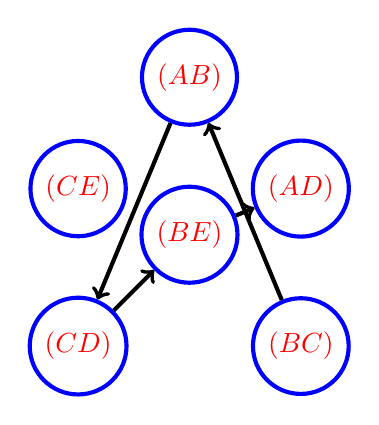
\begin{tikzpicture}[->,node distance = 2cm,line width=1.5pt]
\node[state,text=red,draw=blue] (A) {$(AB)$};
\node[state,text=red,draw=blue] (B) [below left of = A] {$(CE)$};
\node[state,text=red,draw=blue] (D) [below right of = A] {$(AD)$};
\node[state,text=red,draw=blue] (E) [below of = D] {$(BC)$};
\node[state,text=red,draw=blue] (G) [below of = A] {$(BE)$};
\node[state,text=red,draw=blue] (F) [below of = B] {$(CD)$};

\path (A) edge (F);
\path (F) edge (G);
\path (G) edge (D);
\path (E) edge (A);

\end{tikzpicture}
\end{center}

\textcolor{red}{\centerline{\textbf{Fig.4.19} \hspace*{0.5cm} \texttt{Compatible Graph}}}


\hspace*{0.2cm} The states of the minimal machine are $(AD)$, $(CD)$, and $(BE)$. Let us rename them as $S_1$, $S_2$, and $S_3$,
respectively. The minimal machine of this machine is\\


\begin{center}
\begin{tabular}{ccccc}
 \hline

 \hline

 \hline

 \hline

\multicolumn{5}{c}{$Next State, z$}\\
 \cline{2-5}
       $Present State$   &    $I_1$      &    $I_2$        &        $I_3$   &     $I_4$      \\
 \hline
       $S_1(AD)$         &    $S_3, 1$   &     $S_2, 0$    &     $S_1/S_2, 0$   &   $S_2, 0$        \\
       $S_2(CD)$         &    $S_3, 1$   &     $S_2, 0$    &     $S_3, 0$       &   $S_1/S_2, 0$    \\
       $S_3(BE)$         &    $S_1, 1$   &     $-, -$      &     $-, -$         &   $S_1, 1$        \\
 \hline

 \hline

 \hline

 \hline
\end{tabular}
\end{center}

\fcolorbox{blue}{yellow}{\textbf{4.8 \hspace*{0.5cm} Merger Table}}

\vspace*{0.2cm}
The merger table is a substitute application of the merger graph. Similar to the merger graph from the
merger table, we can also get the compatible pairs and implied pairs.\\
\hspace*{0.5cm} If the number of states of a machine increases, the number of combination pair increases. For a machine of n states, the number of two state combinations are $\textcolor[rgb]{1.00,1.00,1.00}{.}^nC_2, i.e$., $n(n-1)/2$. If $n = (n-1)$, the number of combinations are $(n-1)$ $(n-2)/2$. The number of combinations increases to $(n-1)$ if the number of states increases from $(n-1)$ to n. It is difficult to connect two states by arcs if the number of states increases. In substitute of that, the merger table is an easier process to find compatible pairs and implied pairs.\\

\vspace*{0.5cm}

\fcolorbox{blue}{yellow}{\textbf{4.8.1 \hspace*{0.5cm} Construction of a Merger Table}}

\vspace*{0.2cm}
A merger table can be constructed by the following way.\\

\begin{itemize}
  \item Make a table of $(n-1) \times (n-1)$, where the left hand side is labelled by the $2nd$ state to the nth state
and the right hand side is labelled by the 1st state to the $(n-1)$th state.
  \item Each box represents a pair of state combination.
\end{itemize}

\newpage

\begin{flushleft}
 \textcolor{blue}{\textbf{160}\hspace*{0.1cm} \textbf{$|$} \hspace*{0.1cm} \texttt{Introduction to Automata Theory, Formal Languages and Computation}}
  \end{flushleft}


\vspace*{1cm}
\begin{itemize}
  \item Put a cross in the box if the outputs conflict for the pair of states.\\
  \item Put a right sign in the box if the outputs as well as next states do not conflict for the pair of states.\\
  \item If the outputs do not conflict but the next states conflict for the pair of states, put the conflicting
next states in the box.\\
\end{itemize}

The following examples describe the process in detail.\\

\vspace*{0.5cm}

\fcolorbox{red}{pink}{\textcolor[rgb]{0.00,0.00,0.00}{Example 4.12}} \hspace*{0.1cm} \texttt{Construct a merger table of the following machine and find the compatible pairs.}\\

\textbf{Solution:}\\
\begin{center}
\begin{tabular}{cccc}
 \hline

 \hline

 \hline

 \hline

\multicolumn{4}{c}{$Next State, z$}\\
 \cline{2-4}
       $Present State$   &    $I_1$      &    $I_2$        &        $I_3$      \\
 \hline
     $A$ & $E, 0$ & $B, -$ & $C, -$ \\
     $B$ & $-, -$ & $D, -$ & $B, 0$ \\
     $C$ & $E, -$ & $D, -$ & $C, 0$ \\
     $D$ & $C, 0$ & $-, -$ & $B, 1$ \\
     $E$ & $C, 0$ & $-, -$ & $B, -$ \\
 \hline

 \hline

 \hline

 \hline
\end{tabular}
\end{center}

\vspace*{0.2cm}

Make a table like the following:\\

\begin{center}
\section{picture}
\includegraphics[width=4.5cm,height=2.3cm]{160.png}
\end{center}

\hspace*{0.5cm} Consider the state combination (AB). Here, the outputs do not conflict but the next states for $I_2$ and $I_3$
conflict. So, the conflicting next state combinations, (BD) and (BC), are placed in the box labelled (AB).\\
\hspace*{0.5cm} Consider the state combination (AC). Here, the outputs do not conflict but the next states for $I_2$ conflict. So, the conflicting next state combination, (BD), is placed in the box labelled (AC).\\
\hspace*{0.5cm} Consider the state combination (AD). The outputs do not conflict, but the next states for $I_1$ and $I_3$
conflict. The conflicting next state combinations (CE) and (BC) are placed in the box labelled (AD).\\


\hspace*{0.5cm} Consider the state combination (AE). The outputs for the states do not conflict, but the next states for
input $I_1$ and $I_3$ conflict. (CE) and (BC) are placed in the box labelled (AE).\\
\hspace*{0.5cm} Consider the state combination (BD). Here, the outputs for input $I_3$ conflict. There will be an $\times$ (cross)
in the box labelled (BD).\\
\hspace*{0.5cm} Consider state combination (DE). Here, both the outputs and the next state combination are the same
for all the inputs. So a $ \surd$ (tick) is placed in the box labelled (DE).\\

\end{document} 